%\chapter{Bahnplanung} 
\chapter{Implementierung der Via-Punkt Trajektorie}
%\section{Bahnplanungsansätze im Vergleich}
%\section{Analyse und Approximation der KUKA Bahnplanung}
%\section{Implementierung der Via-Punkt Trajektorie}
Die Berechnung der Bewegungsbahn erfolgt für alle sechs Gelenkwinkel $\theta_i$ nach demselben Ansatz, einem Polynom sechster Ordnung. 
%
\begin{align}
	\theta(t) &= a_0 + a_1t + a_2t^2 + a_3t^3 + a_4t^4 + a_5t^5  + a_6t^6 \\
	\dot{\theta}(t) &= a_1 + 2a_2t + 3a_3t^2 + 4a_4t^3 + 5a_5t^4  + 6a_6t^5\\
	\ddot{\theta}(t) &= 2a_2 + 6a_3t + 12a_4t^2 + 20a_5t^3  + 30a_6t^4
\end{align}
%
Maßgeblich für die Ordnung des Polynoms ist die Anzahl von sieben Nebenbedingungen.  Definiert sind der Startwinkel $\theta_i(t_s)$, die Anfangsgeschwindigkeit $\dot{\theta}_i(t_s) = 0$, die Anfangsbeschleunigung $\ddot{\theta}_i(t_s) = 0$, der Via-Punkt-Winkel $\theta_i(t_v)$, sowie der Winkel im Zielpunkt $\theta_i(t_e)$, die Endgeschwindigkeit $\dot{\theta}_i(t_e) = 0$ und die Endbeschleunigung $\ddot{\theta}_i(t_e) = 0$. Darüber hinaus sind der Startzeitpunkt $t_s$, der Zeitpunkt für das Erreichen des Via-Punkts, sowie die Dauer der Bewegung über den Endzeitpunkt $t_e$ vorgegeben. 
%
Die Bestimmung der Parameter $a_0, ... a_6$ erfolgt durch Lösen des linearen Gleichungssystems \ref{eqn:lgs}. Die Implementierung in MATLAB\textsuperscript{\textregistered} ist im Anhang \ref{add:traj} hinterlegt.
%
\begin{equation}
	\label{eqn:lgs}
	\left[	\begin{matrix}
		1&\quad    t_s&\quad          	t_s^2&\quad              	t_s^3&\quad         	t_s^4&\quad              	t_s^5&\quad          	t_s^6\\
		0&\quad    t_s&\quad          	2t_s&\quad              	3t_s^2&\quad        	4t_s^3&\quad            	5t_s^4&\quad        	6t_s^5\\
		0&\quad    0&\quad         		2&\quad              	  	6t_s&\quad         	 	12t_s^2&\quad           	20t_s^3&\quad       	30t_s^4\\
		1&\quad    t_v&\quad         	t_v^2&\quad              	t_v^3&\quad         	t_v^4&\quad             	t_v^5&\quad          	t_v^6\\
		1&\quad    t_e&\quad        	t_e^2&\quad              	t_e^3&\quad          	t_e^4&\quad             	t_e^5&\quad          	t_e^6\\
		0&\quad    1&\quad   	   		2t_e&\quad              	3t_e^2&\quad        	4t_e^3&\quad           		5t_e^4&\quad        	6t_e^5\\   
		0&\quad    0&\quad          	2&\quad                 	6t_e&\quad          	12t_e^2&\quad           	20t_e^3&\quad       	30t_e^4
	\end{matrix}\right]
	\left[	\begin{matrix}
		a_0\\
		a_1\\
		a_2\\
		a_3\\
		a_4\\
		a_5\\
		a_6\\		
	\end{matrix}\right] = 
		\left[	\begin{matrix}
		\theta_s\\
		\dot{\theta}_s\\
		\ddot{\theta}_s\\
		\theta_v\\
		\theta_e\\
		\dot{\theta}_e\\
		\ddot{\theta}_e\\		
	\end{matrix}\right]
\end{equation}
%
Die Bestimmung der Roboterdynamik setzt voraus, dass die berechnete Bewegungsbahn $\theta(t)$, sowie die dazugehörigen Verläufe $\dot{\theta}(t) ~\ddot{\theta}(t)$  die, von der KUKA Robotersteuerung berechnete Trajektorie möglichst genau approximieren. Hierzu wird eine Bewegung aus dem Programm $Kleben-Seitenwand$, welches auf der KRC5 des Roboters abgelegt ist und bereits für den Roboter auf Kollisionsfreiheit validiert ist, getestet. Die Bewegung ist in der Bewegungsart  Punkt-zu-Punkt (Point-To-Point)(PTP)) programmiert und sieht vor, den Roboter von dem letzten Prozesspunkt auf seine Warteposition (Home-Position) zu verfahren. Die Start- und Zielwinkel sind wie folgt definiert. Die MATLAB\textsuperscript{\textregistered}-Implementierung der Bewegung im Anhang \ref{add:sim} hinterlegt.
%Die Abbildungen \ref{fig:gelenkwinkel}
Startwert Gelenkwinkel\\
$\theta_{s1} = -53,8$\\
$\theta_{s2} = -70,34^{\circ}$\\
$\theta_{s3} = 98,82-90^{\circ}$\\
$\theta_{s4} = -69,87^{\circ}$\\  
$\theta_{s5} = -58,7^{\circ}$\\ 
$\theta_{s6} = 55,7^{\circ}$\\
%
Zielwert Gelenkwinkel\\
$\theta_{e1} = -7,61^{\circ}$\\     
$\theta_{e2} = -119,27^{\circ}$\\      
$\theta_{e3} = 88,49-90^{\circ}$\\ 
$\theta_{e4} = 10,27^{\circ}$\\
$\theta_{e5} = 32,41^{\circ}$\\   
$\theta_{e6} = -10,19^{\circ}$\\         
%
Startwert Via-Punkte\\
$\theta_{v1}$ = $\tfrac{\theta_{s1}+\theta_{e1}}{2}$\\
$\theta_{v1}$ = $\tfrac{\theta_{s2}+\theta_{e2}}{2}$\\
$\theta_{v1}$ = $\tfrac{\theta_{s3}+\theta_{e3}}{2}$\\
$\theta_{v1}$ = $\tfrac{\theta_{s4}+\theta_{e4}}{2}$\\
$\theta_{v1}$ = $\tfrac{\theta_{s5}+\theta_{e5}}{2}$\\
$\theta_{v1}$ = $\tfrac{\theta_{s6}+\theta_{e6}}{2}$\\
%
Die Abbildungen \ref{fig:gelenkwinkel}, \ref{fig:winkelgeschwindigkeit} und  \ref{fig:winkelbeschleunigung}  visualisieren die simulierte Bewegung. \ref{fig:gelenkwinkelpy} zeigt den zeitlichen Verlauf der Gelenkwinkel am realen System. Die Daten sind mit einem einem  Zeitabstand $\Delta t = 4~ms$ abgetastet. Für Visualisierung der Winkelgeschwindigkeit  erfolgt zunächst die Bildung des Differenzenquotienten für zwei benachbarte Abtastwerte. Durch eine anschießende Tiefpassfilterung wird der zeitliche Verlauf geglättet, siehe Abbildung \ref{fig:winkelgeschwindigkeit_py1}. Die Abtastfrequenz beträgt 250 Hz. Die Eckfrequenz des Butterworth-Filters wird auf 10 Hz definiert. Die Daten der Winkelbeschleunigung werden für dasselbe Vorgehen durch Bildung des zentralen Differenzenquotienten für die zweite Ableitung berechnet.


 \ref{fig:winkelgeschwindigkeit_py1}, \ref{fig:winkelbeschleunigung_py} die zeitlichen Verläufe der implementierten Trajektorien mit den, von der KUKA Robotersteuerung berechneten Bahnverläufen verglichen.
%
\newpage
\begin{figure}[]
	\centering
	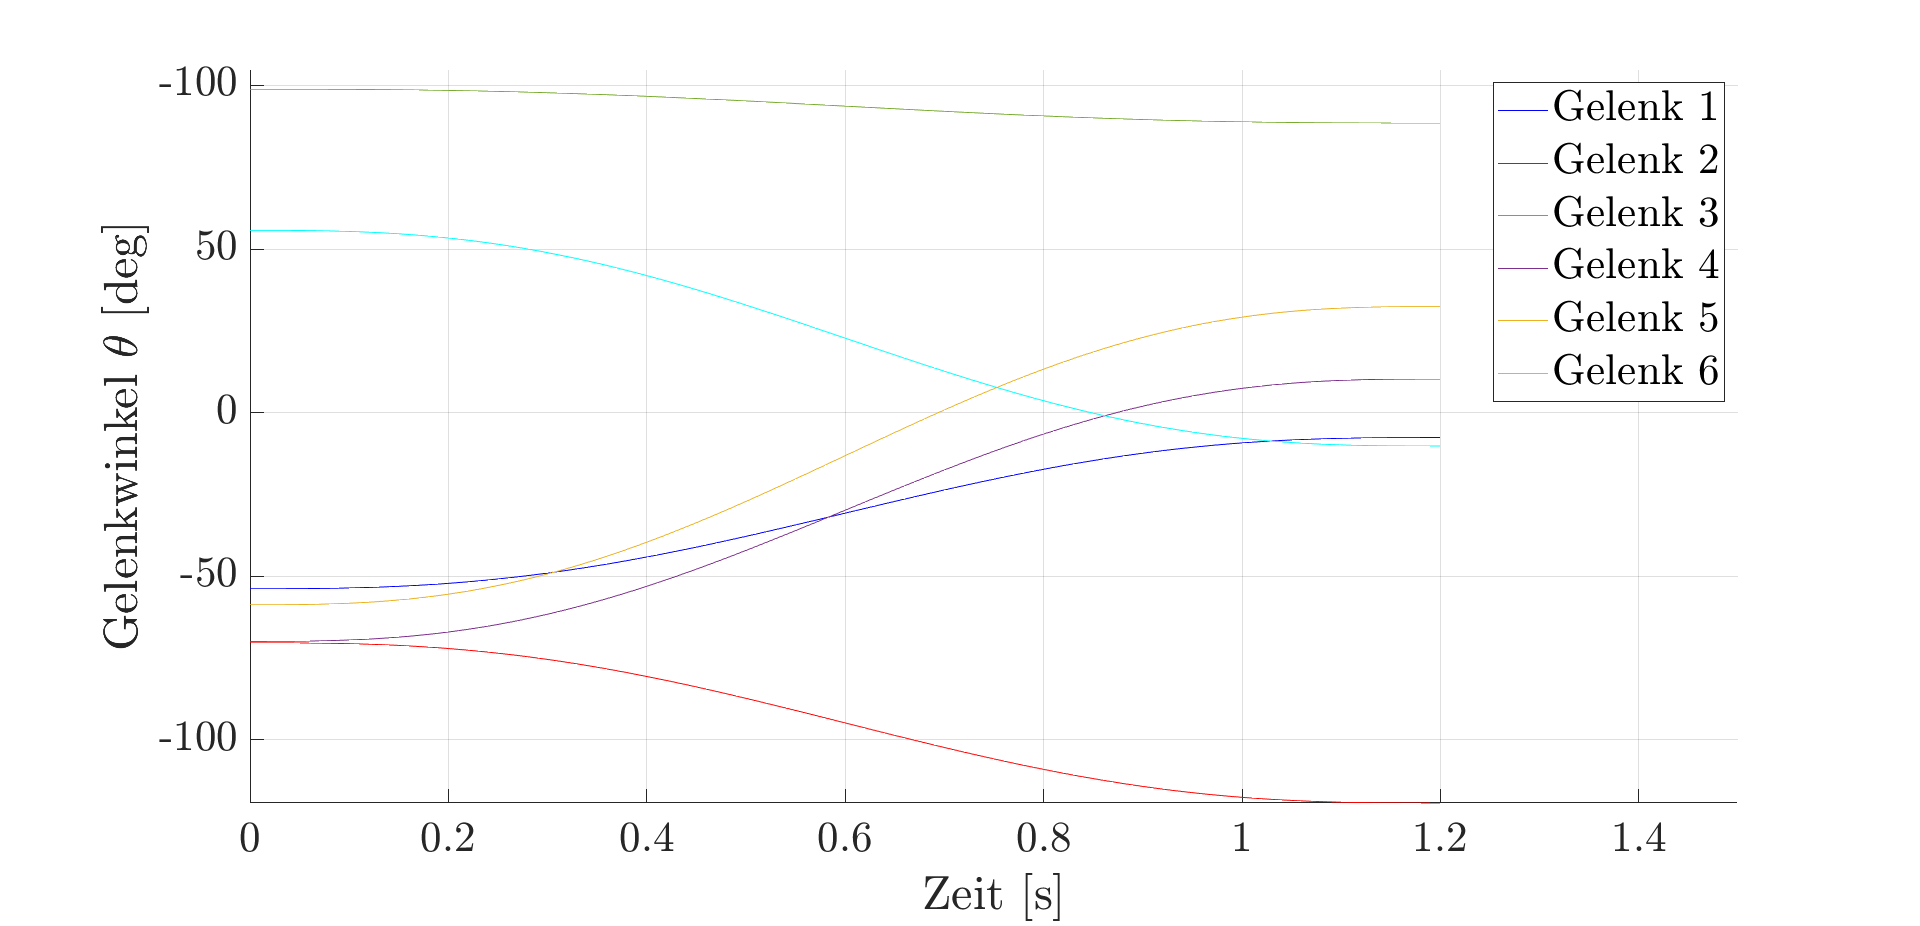
\includegraphics[width=1\linewidth]{images/gelenkwinkel}
	\caption{Gelenkwinkel}
	\label{fig:gelenkwinkel}
\end{figure}
%
\begin{figure}[]
	\centering
	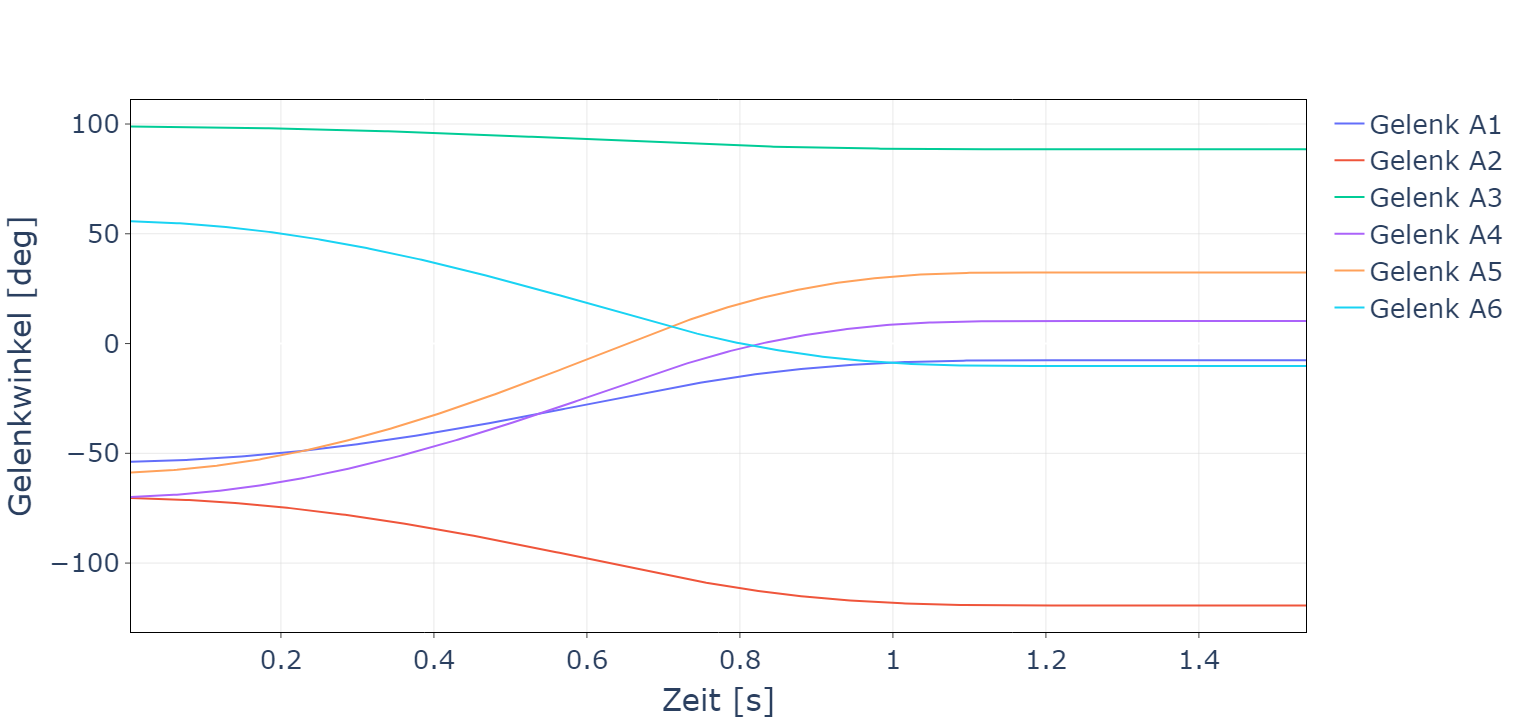
\includegraphics[width=1\linewidth]{images/gelenkwinkel_py}
	\caption{Gelenkwinkel}
	\label{fig:gelenkwinkelpy}
\end{figure}
%
\newpage
\begin{figure}[]
	\centering
	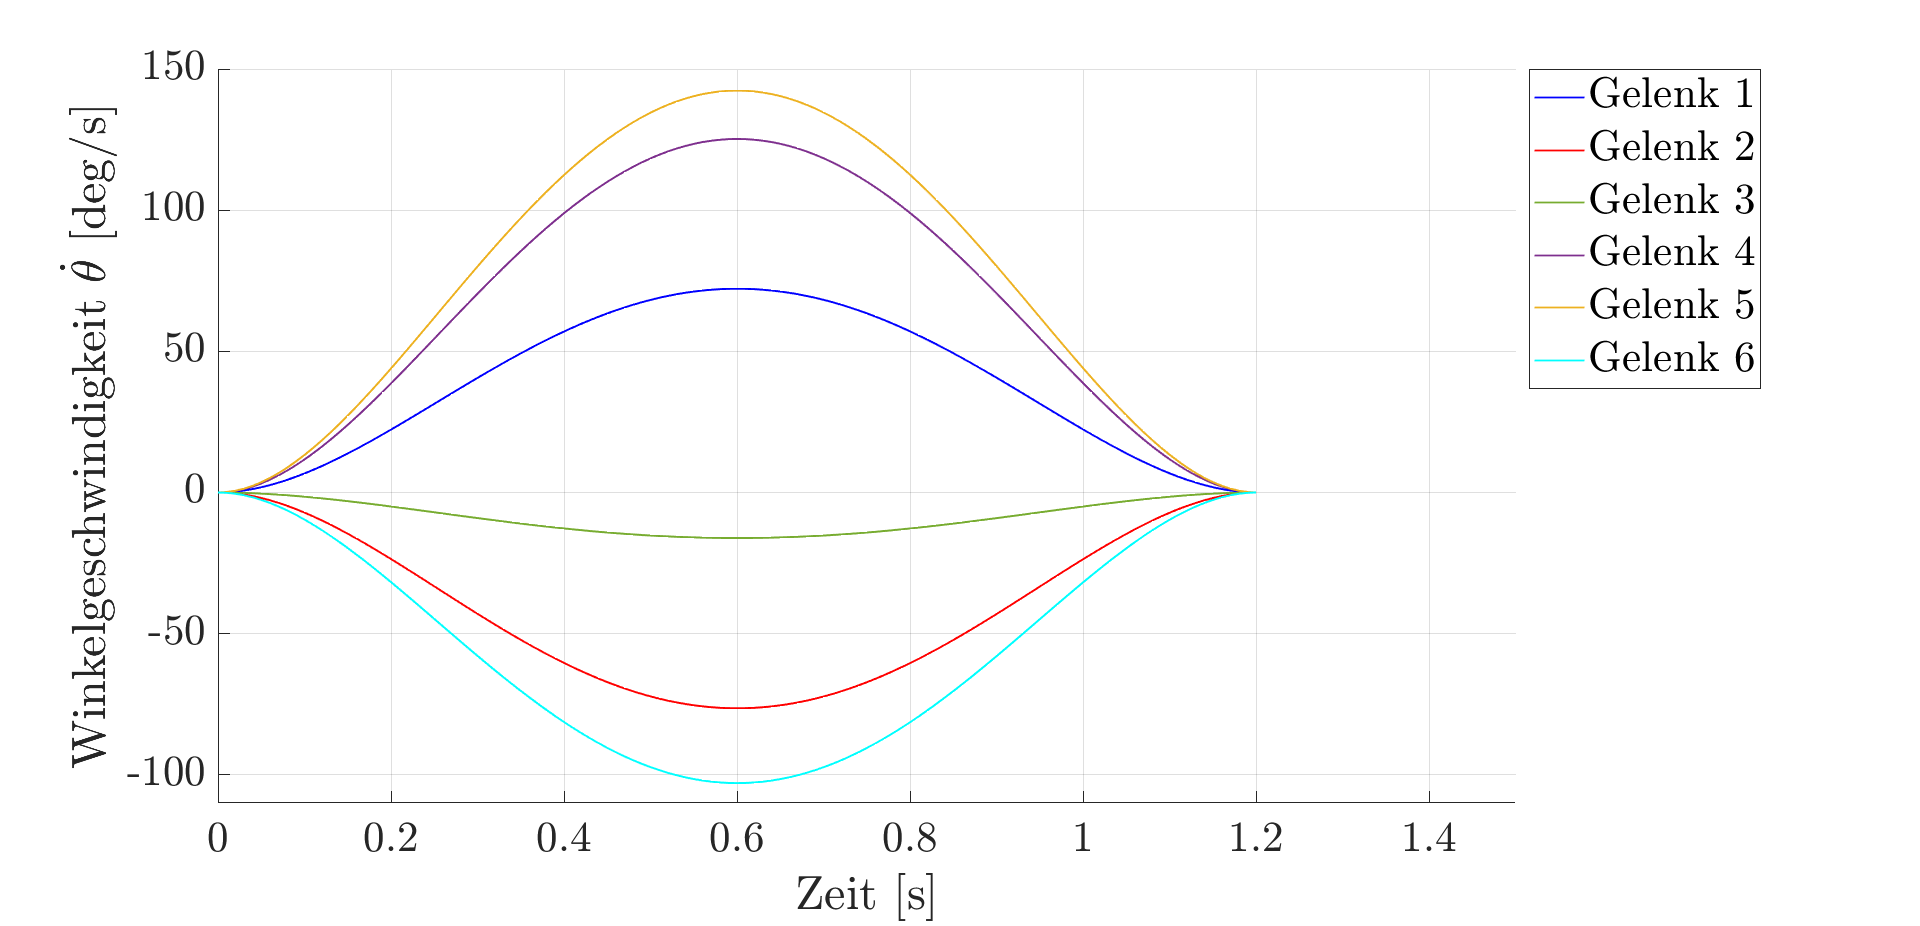
\includegraphics[width=1\linewidth]{images/winkelgeschwindigkeit}
	\caption{Winkelgeschwindigkeit}
	\label{fig:winkelgeschwindigkeit}
\end{figure}
%
\begin{figure}[]
	\centering
	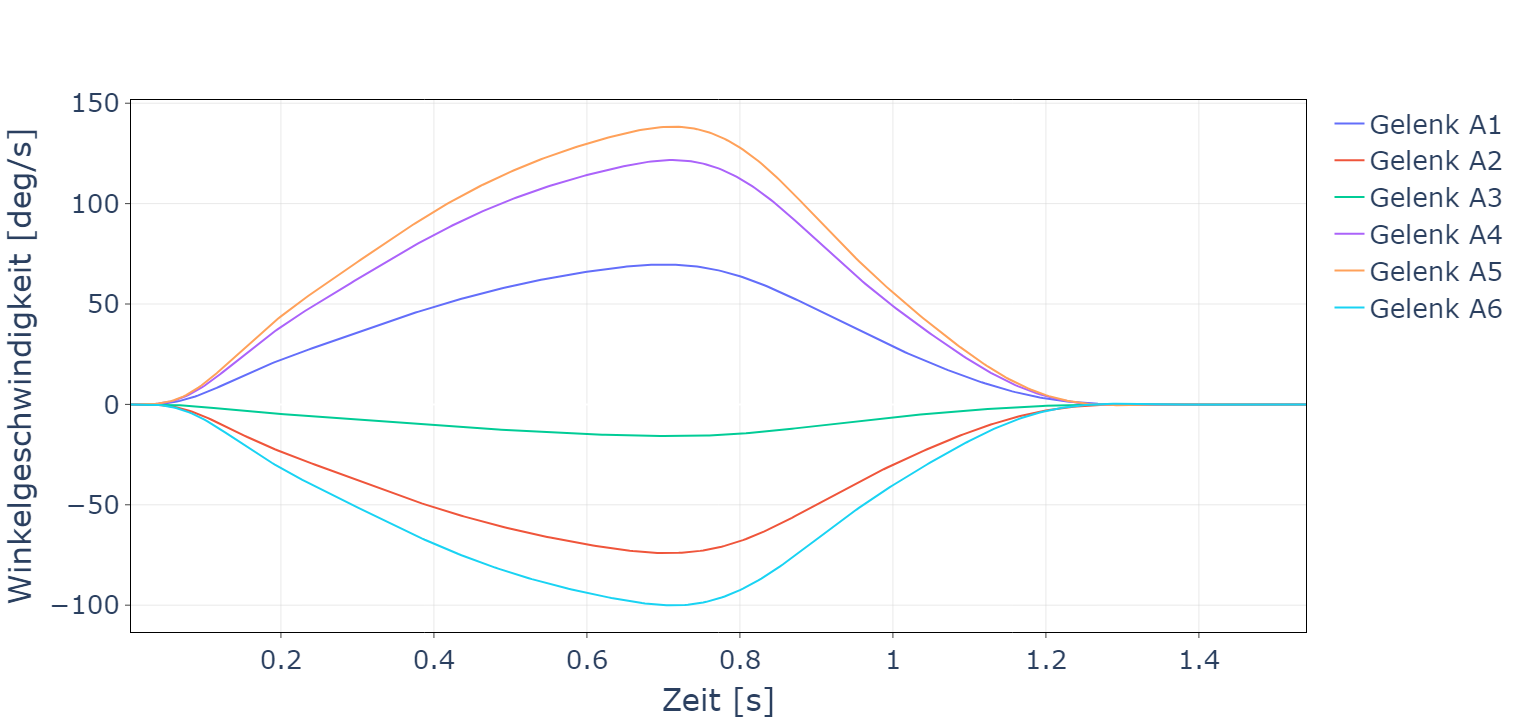
\includegraphics[width=1\linewidth]{images/winkelgeschwindigkeit_py}
	\caption{Winkelgeschwindigkeit}
	\label{fig:winkelgeschwindigkeit_py1}
\end{figure}
%
\newpage
\begin{figure}[]
	\centering
	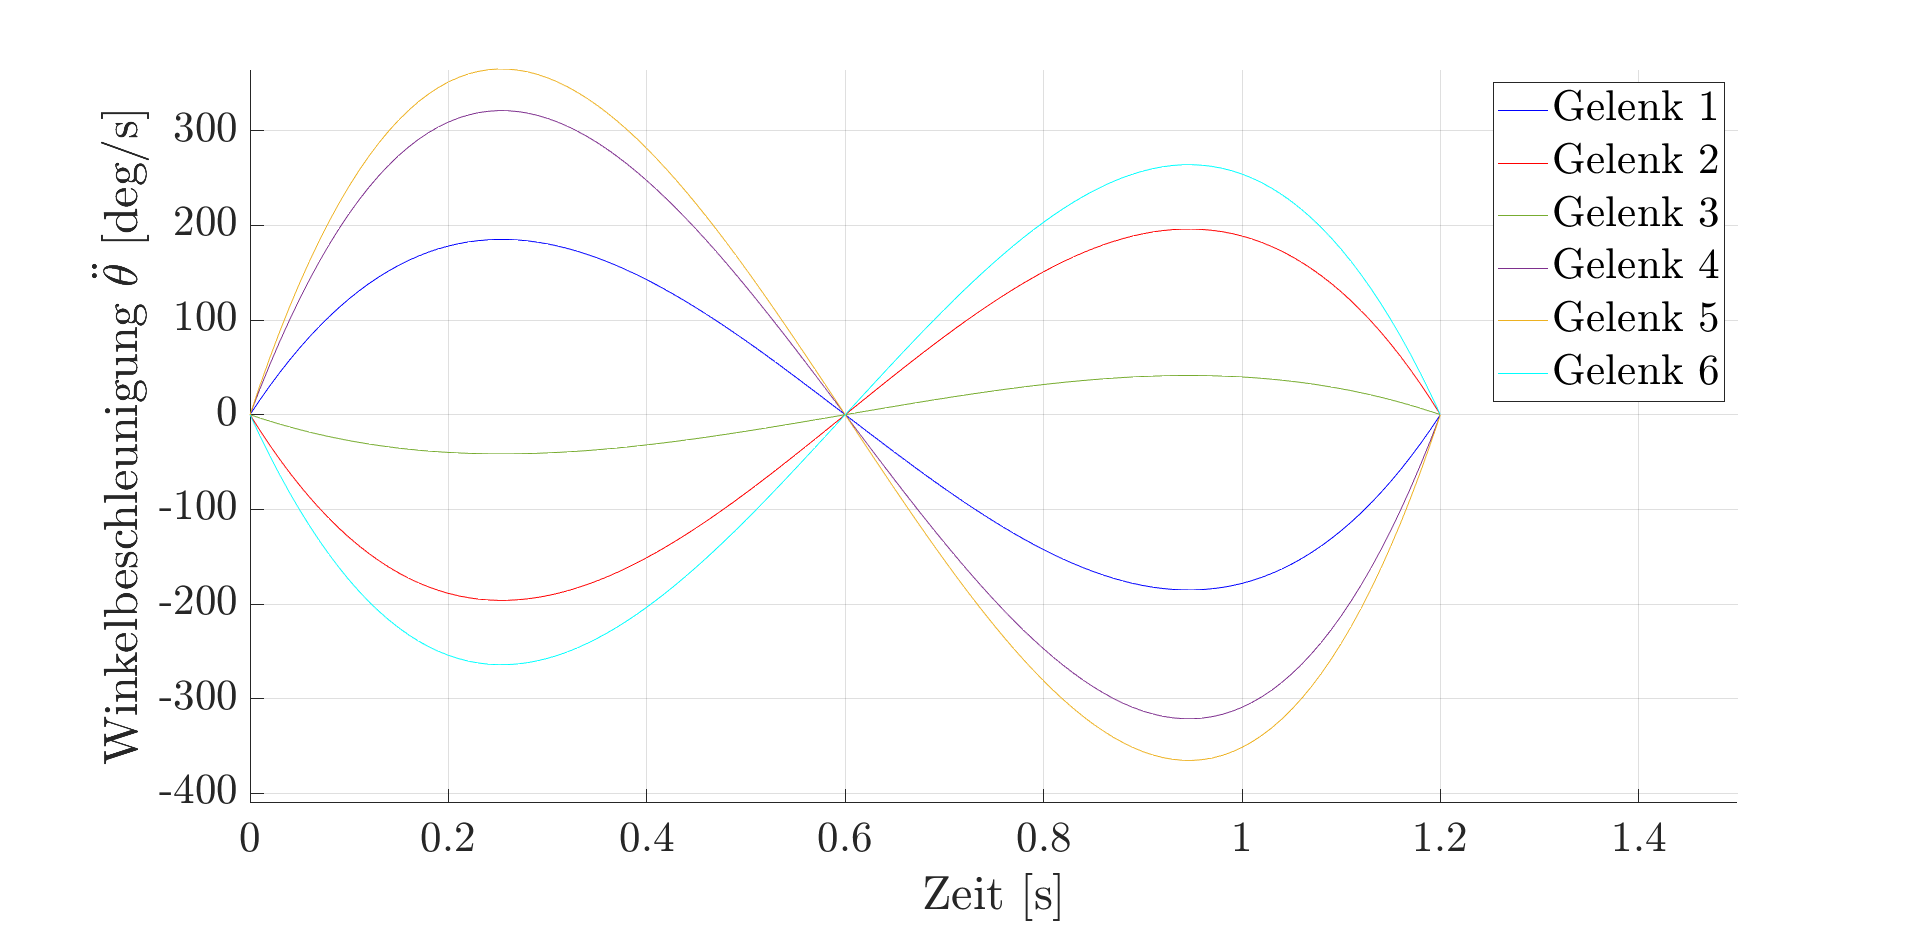
\includegraphics[width=1\linewidth]{images/winkelbeschleunigung}
	\caption{Winkelbeschleunigung}
	\label{fig:winkelbeschleunigung}
\end{figure}
%
\begin{figure}[]
	\centering
	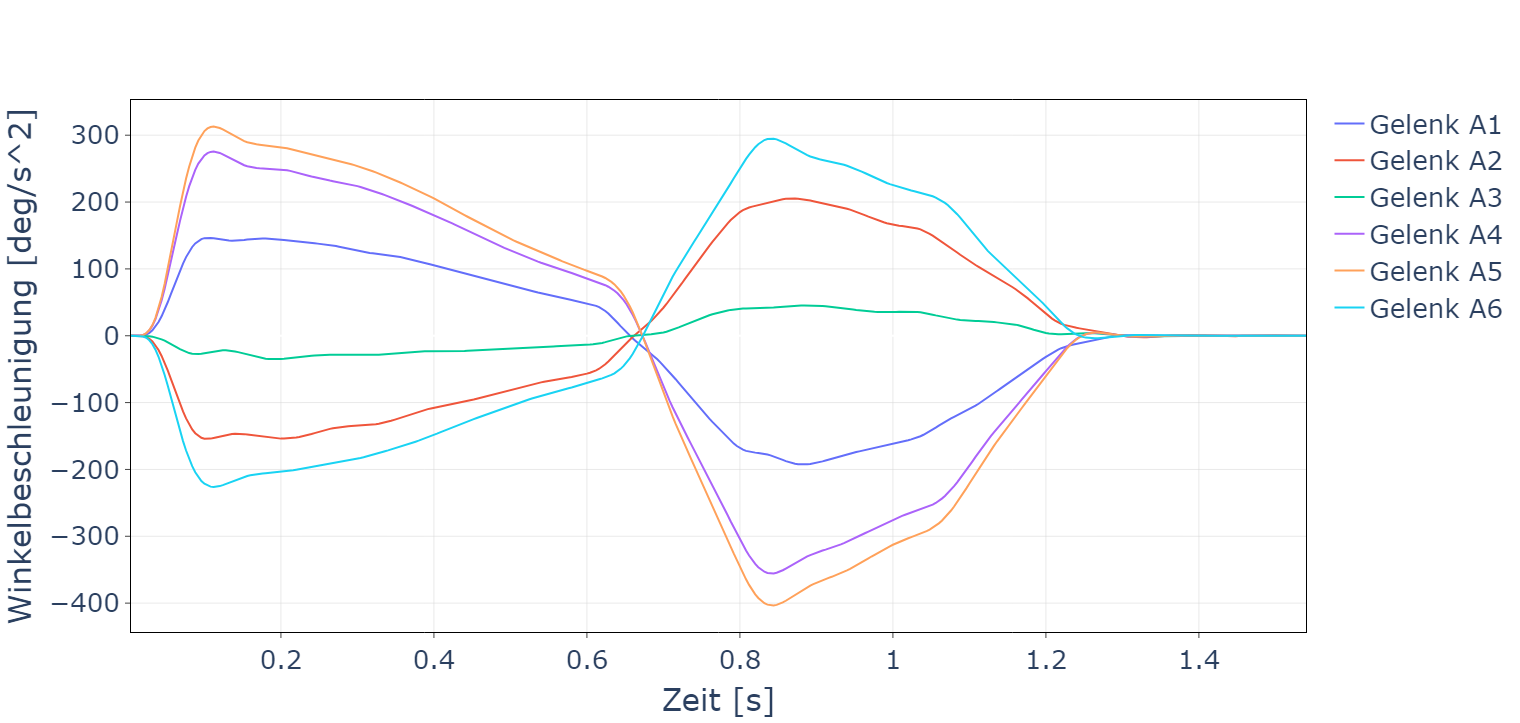
\includegraphics[width=1\linewidth]{images/winkelbeschleunigung_py1}
	\caption{Winkelbeschleunigung}
	\label{fig:winkelbeschleunigung_py}
\end{figure}
